\documentclass{article}

\usepackage[utf8]{inputenc} % allow utf-8 input
\usepackage[T1]{fontenc}    % use 8-bit T1 fonts
\usepackage{url}            % simple URL typesetting
\usepackage{booktabs}       % professional-quality tables
\usepackage{amsfonts}       % blackboard math symbols
\usepackage{nicefrac}       % compact symbols for 1/2, etc.
\usepackage{microtype}      % microtypography
\usepackage{graphicx}
\usepackage{ml4cps}         % Load the custom style FIRST
\usepackage[numbers,sort&compress]{natbib} % numeric cites, auto-sort/compress
\usepackage[hidelinks]{hyperref}           % load AFTER natbib
\usepackage{doi}
\usepackage{amsmath}
\usepackage[nameinlink,noabbrev]{cleveref} % load AFTER hyperref
\usepackage{tabularx}       % for wrapping text in tables
\usepackage{array}

\title{A Production-Grade Intrusion Detection System with Cloud-Native MLOps}

\date{}

\newif\ifuniqueAffiliation
% Uncomment to use multiple affiliations variant of author block 
\uniqueAffiliationtrue

\ifuniqueAffiliation % Standard variant of author block
\author{
    \href{https://orcid.org/0009-0002-9752-0688}{
\includegraphics[scale=0.06]{orcid.pdf}\hspace{1mm}Vince Mbanze}\\
    MLOps Engineer, Nexusnode\\
    \texttt{vince.mbanze@nexusnode.co.za} \\
    \And
    Thabo Pilusa \\
    Software Developer, Nexusnode \\
    \texttt{thabo.pilusa@nexusnode.co.za} \\
}
\else
% Multiple affiliations variant of author block
\usepackage{authblk}
\renewcommand\Authfont{\bfseries}
\setlength{\affilsep}{0em}
% box is needed for correct spacing with authblk
\newbox{\orcid}\sbox{\orcid}{
\includegraphics[scale=0.06]{orcid.pdf}} 
\author[1]{%
	\href{https://orcid.org/0000-0000-0000-0000}{\usebox{\orcid}\hspace{1mm}First author}%
}
\author[1,2]{%
	\href{https://orcid.org/0000-0000-0000-0000}{\usebox{\orcid}\hspace{1mm}Second author}%
}
\affil[1]{Affiliation, Address}
\affil[2]{Affiliation, Address}
\fi

\renewcommand{\shorttitle}{Production-Grade IDS with MLOps}

%%% Add PDF metadata to help others organize their library
\hypersetup{
pdftitle={A Production-Grade Intrusion Detection System with Cloud-Native MLOps},
pdfsubject={Intrusion Detection, MLOps},
pdfauthor={Vince Mbanze, Thabo Pilusa},
pdfkeywords={Intrusion Detection System, MLOps, XGBoost, ONNX, Kubernetes, FastAPI, CI/CD},
}

\begin{document}

\maketitle

\begin{abstract}
We present an end-to-end intrusion detection system (IDS) on the UNSW-NB15 dataset, engineered for production. The pipeline produces 34 numeric features via reproducible cleaning, encoding, and scaling; models are tuned on a train/validation split and evaluated on a held-out test set. Among logistic regression, a multilayer perceptron, random forest, and gradient-boosted trees, XGBoost delivered the best recall–precision trade-off. On the test set, the final model achieved a Receiver Operating Characteristic Area Under the Curve (ROC-AUC) of 0.9805. At a high-recall operating point ($\tau=0.6286$) chosen to minimize the False Positive Rate (FPR) subject to recall $\ge 0.95$, the model reached an F1-score of 0.9101, precision of 0.8708, and recall of 0.9531. The trained model is exported to the Open Neural Network Exchange (ONNX) format and served with onnxruntime behind a token-authenticated Application Programming Interface (API) microservice, with a Dash User Interface (UI) for ad-hoc scoring and threshold management. For production, we containerize the API and UI and deploy on Amazon Elastic Kubernetes Service (EKS) via Kustomize overlays; GitHub Actions workflows manage integration via Docker Hub and deployment to Amazon Elastic Container Registry (ECR), run smoke tests, and execute rollouts with readiness/liveness probes and a Horizontal Pod Autoscaler (HPA). Secrets are managed via Kubernetes Secrets.
\end{abstract}

% add keywords
\keywords{Intrusion Detection System (IDS) \and MLOps \and XGBoost \and ONNX \and Kubernetes}

\section{Introduction}
Intrusion detection remains foundational for securing contemporary networks, but real-world value depends as much on operational reliability as on classifier accuracy. Production environments are high-throughput, elastic, and heterogeneous: traffic mixes shift, the base rate of attack is low and non-stationary, and the cost of misses typically dominates the cost of additional triage. An effective IDS must therefore pair strong discrimination on historical data with stable behaviour under workload variation, transparent failure modes, and operator controls for responsible tuning \cite{cho2009}.

Much of the IDS literature stops short of deployability. Studies optimise models offline on public corpora and report headline scores, while leaving unresolved the issues that determine whether a system can run in anger: keeping the feature space consistent between training and serving; choosing decision thresholds by a principled cost model that remains sensible as prevalence shifts; guaranteeing that the artefact evaluated in research is the same one served to users; and managing updates, rollbacks, health checks, and autoscaling so detection remains available through traffic spikes and partial infrastructure failure \cite{apruzzese2023, landauer2022}.

This work addresses that research-to-operations gap. Our goal is not a novel classifier, but a governable one which is measurable, reproducible, and adjustable under changing conditions. Concretely, we ground the study in a widely used benchmark for comparability, yet treat the dataset as a means rather than the end. The core contribution is an auditable evidence chain spanning data transformations, model artefacts, serving contract, and operational controls in a form a third party can verify and operate \cite{bertoli2021, kim2012}.

\subsection*{Contributions}
\begin{itemize}
    \item \textbf{Feature/serve alignment.} A reproducible feature pipeline with a strict schema contract, ensuring the vectors used in training are identically realised at serve time.
    \item \textbf{Operating-point governance.} An auditable procedure for threshold selection that encodes operational costs (e.g., minimum recall subject to low false-positive rate), with mechanisms to revise the threshold safely as base rates drift \cite{strasburg2016}.
    \item \textbf{Portability \& parity.} Export of the trained model to ONNX with parity checks that verify train–serve consistency across runtimes.
    \item \textbf{Service interface \& observability.} A token-authenticated API exposing probabilistic and hard-label predictions, paired with an operator UI for inspection and threshold management; health and readiness probes to enable safe rollouts and autoscaling \cite{dreger2007}.
    \item \textbf{Release discipline.} CI/CD gates (tests, smoke checks, and rollback hooks) that prevent configuration or parity regressions from reaching users \cite{shaikh2009}.
\end{itemize}

We then situate the approach among prior IDS and deployment work, describe the dataset and evaluation protocol, present the model and operating-point rationale, report empirical results with attention to calibration and error profiles, and detail the system properties including reproducibility, portability, health, scaling, and release discipline, which make the IDS suitable for cloud environments.

\section{Related Work}
Classical IDSs fall into two broad paradigms, namely: misuse (signature-based) and anomaly-based detection. Signature systems such as rule engines achieve high precision on known threats but generalise poorly to novel or obfuscated attacks. Anomaly-based methods learn a model of “normal” behaviour and flag deviations; they offer novelty sensitivity but are prone to false alarms when workload or configuration shifts \cite{wong2007}. Machine-learning IDSs attempt to bridge this gap by learning discriminative mappings from traffic features to attack labels, typically at the flow or session level, but their deployability often hinges on choices, such as feature stability, thresholding, and calibration that receive limited attention in the literature \cite{bhardwaj2013, subbulakshmi2009}.

Benchmark datasets have shaped the field and its pitfalls. Early corpora (e.g., KDD and NSL-KDD) are now known to contain artefacts that inflate accuracy \cite{silva2020}, motivating more recent sets such as UNSW-NB15 and CIC-IDS families \cite{abdulraheem2019, sharafaldin2018}. Even with improved curation, evaluation protocols frequently mix flows from the same capture across train and test, obscuring temporal shift as metrics are reported at a single, sometimes implicit threshold and without prevalence sensitivity, and leakage through target-correlated categorical encodings remains a recurrent issue \cite{viegas2017}. Work on class imbalance (reweighting, sampling) and cost-sensitive learning alleviates some effects but does not by itself resolve operating-point selection under changing base rates.

Across modelling approaches, tree ensembles (random forests, gradient-boosted trees) remain strong baselines for tabular traffic features, often matching or exceeding deep architectures while offering better latency and interpretability \cite{abedin2018}. Deep models, such as CNNs/LSTMs, on flow sequences, autoencoders for unsupervised detection, and graph or attention models for higher-order structure—have broadened the design space \cite{clausen2020, glavan2023}, yet gains are uneven once rigorous splits, calibration, and cost-aware thresholds are enforced. Post-hoc explanation methods (e.g., SHAP) are increasingly used to probe feature influence, but they are rarely integrated into the operational controls of a live system \cite{spadari2024}.

A small but growing body of work addresses serving and operations. Prior studies have explored model export to portable formats and microservice deployment, but many stop at containerisation without specifying health probes, resource governance, autoscaling, or release gates \cite{catillo2025}. Production systems outside academia routinely rely on model servers (e.g., ONNX Runtime, TensorFlow Serving) behind authenticated APIs, with schema contracts, parity tests, and CI/CD gates; however, these practices are seldom documented alongside IDS research results \cite{srivastav2022}. As a consequence, the literature often conflates model promise with system reliability.

This study situates itself at that intersection. Rather than proposing a new classifier, we synthesise established ingredients which include tabular features, gradient-boosted trees, portable model export into a specification that targets the missing operational layer: strict train–serve feature alignment, auditable threshold selection, numerical parity checks across runtimes, and a cloud deployment that makes availability, scaling, and rollback first-class concerns.

\subsection*{Comparative summary}
\Cref{tab:comparison} contrasts representative UNSW-NB15 studies along the axes that determine deployability: split discipline, threshold/calibration awareness (as reflected by reported metrics), and whether serving/operations are documented. Five of six studies report accuracy as a primary figure, only one reports ROC-AUC, and none document threshold governance or serving except this work, which couples ROC-family metrics with an auditable operating point and a production interface.

\begin{table}[ht!]
\caption{Experimental setup comparison across UNSW-NB15 IDS studies. “Deployment/Serving” refers to any documented portable export, API, health probes, or CI/CD checks.}
\label{tab:comparison}
\centering
\renewcommand{\arraystretch}{1.6}
\begin{tabularx}{\textwidth}{l X X X X X}
\toprule
\textbf{Study} & \textbf{Dataset Protocol} & \textbf{Models} & \textbf{Metrics} & \textbf{Deployment / Serving} & \textbf{Source}\\
\midrule
This work (2026) & UNSW-NB15 fixed splits; stratified validation; reproducible preprocessing & LR, MLP, RF, XGBoost & ROC-AUC, Precision, Recall, F1, FPR, Confusion matrix & ONNX export, FastAPI service, CI/CD smoke tests, threshold governance & -\\
\addlinespace
Kocher \& Kumar (2020)  & UNSW-NB15, standard ML split & NB, LR, KNN, SVM, DT, RF & Accuracy, MSE, Precision, Recall, F1, TPR/FPR & None (offline) & \cite{kocher2020}\\
\addlinespace
Meftah et al. (2019)  & UNSW-NB15, two-stage hybrid classification & SVM, RF (hybrid) & Accuracy, F1, detection rate & None (offline) & \cite{meftah2019}\\
\addlinespace
Kotecha et al. (2021)  & UNSW-NB15, feature correlation/variance analysis & Multiple models, feature-selection guided & Accuracy, Precision, Recall, F1 & None (offline) & \cite{kotecha2021}\\
\addlinespace
Udurume et al. (2024)  & UNSW-NB15 + NSL-KDD, comparative evaluation & CNN, CNN-BiLSTM, KNN, SVM, MLP, RF, DT, LR & Accuracy, Precision, Recall, F1 & None (research comparison) & \cite{udurume2024}\\
\addlinespace
Pinto et al. (2024) & UNSW-NB15 re-exported with HERA from PCAPs & Data regeneration focus & Accuracy across flow versions; export impact & Data preprocessing pipeline focus (not live serving) & \cite{pinto2024}  \\
\bottomrule
\end{tabularx}
\end{table}

\subsection*{Takeaways}
\begin{itemize}
    \item[(i)] Evaluation remains largely accuracy-centric, with limited prevalence-sensitive reporting;
    \item[(ii)] split protocols are often “standard ML splits” rather than fixed published partitions;
    \item[(iii)] serving/ops (schema contracts, health probes, autoscaling, CI gates) are almost never reported. Our study fills this gap by making the operating point and serving contract first-class, and by providing parity checks between research and deployment artefacts.
\end{itemize}

In contrast, our study reports ROC-AUC and operating-point metrics selected under a recall constraint, exports the model to ONNX with parity checks, and documents a token-authenticated API with CI/CD gates and health probes.

\section{Materials and Methods}
\subsection{Data}
We base the study on the UNSW-NB15 intrusion-detection corpus (flow records with attack/normal labels). We use the published training and test partitions as-is ($\approx$ 175,341 train; 82,332 test) to avoid temporal co-mixing \cite{meftah2019}. Records are treated at the flow level, and the binary target is the dataset’s \texttt{label} field (attack vs normal). The auxiliary categorical field \texttt{attack\_cat} is retained for descriptive analyses but excluded from the predictor set.

\textbf{Provenance.} Data were obtained from the Kaggle-hosted UNSW-NB15 corpus (https://www.kaggle.com/datasets/dhoogla/unswnb15/data), a mirror of the original UNSW release.

\textbf{Split discipline.} Within the published training partition we create a stratified validation split on the binary target (fixed seed) for model selection. To prevent count inflation while preserving partition semantics, we remove exact duplicate rows within the training split only; the test split is left untouched. No cross-partition deduplication or temporal reshuffling is performed. Similar disciplined preprocessing has been recommended to improve reliability of UNSW-NB15 evaluations \cite{kocher2020}.

\subsection{Feature engineering}
Feature processing follows the repository’s \texttt{ids\_unsw/features/engineer.py}:
\begin{itemize}
    \item \textbf{Categoricals (processed vs used).} Fields processed as categorical are \texttt{proto}, \texttt{service}, \texttt{state}, and \texttt{attack\_cat}; only \texttt{proto}, \texttt{service}, and \texttt{state} enter the 34-feature predictor set. The \texttt{service} sentinel ``-'' is normalised to ``unknown''.
    \item \textbf{Deterministic encoding.} We use \texttt{OrdinalEncoder(handle\_unknown="use\_encoded\_value", unknown\_value=-1)} fitted on the training split and applied unchanged to validation/test, ensuring unseen symbols map deterministically to -1. %We do not one-hot encode.
    \item \textbf{Numerics \& dtype.} All predictors are numeric and encoded categorical are cast to \texttt{float32}.
    \item \textbf{Scaling.} A \texttt{StandardScaler} is fitted on training and applied to validation/test and at serve time.
    \item \textbf{Schema contract.} The ordered predictor list (34 features) is persisted to \texttt{feature\_names.json}. Cleaned design matrices are materialised as \texttt{UNSW\_NB15\_train\_clean.parquet} and \texttt{UNSW\_NB15\_test\_clean.parquet}.
    \item \textbf{Missingness.} The selected features are complete; no NaNs remain after cleaning.
    \item \textbf{Serve-time expectation.} The live API accepts only the numeric 34-feature schema; categorical text is not accepted.
\end{itemize}
Deterministic encodings and schema contracts address reproducibility and prevent leakage, a recurring challenge in IDS evaluation \cite{alani2021}.

\subsection{Model training}
We treat intrusion detection as binary classification (normal vs attack) on the 34-feature schema and evaluate $\ell_2$-regularised logistic regression, a shallow MLP, random forest, and XGBoost.

\textbf{Class imbalance — two levels.} At the model level, we apply class weighting (e.g., XGBoost \texttt{scale\_pos\_weight} $\approx N_{\text{neg}}/N_{\text{pos}}$; Torch \texttt{pos\_weight}). At the decision level, we choose an operating threshold via a recall-constrained sweep.

\textbf{Tuning.} For XGBoost we use \texttt{hist}/\texttt{gpu\_hist} with early stopping on validation; bounded random search explores tree depth, learning rate, boosting rounds, subsample/colsample, \texttt{min\_child\_weight}, and L1/L2 regularisation. Baselines use small, model-appropriate grids.

\textbf{Operating point.} We minimise FPR subject to recall $\ge 0.95$, breaking ties by precision and then higher thresholds. The same policy is applied on the test split for final reporting.

\textbf{Reproducibility.} All randomised routines use fixed seeds; artefacts (encoder, scaler, model) are persisted.

Comparable model selections and imbalance handling appear across UNSW-NB15 IDS benchmarks \cite{kocher2020, mohamed2023}.

\subsection{Export and validation}
The champion XGBoost model is exported to ONNX with \texttt{onnxmltools}/\texttt{skl2onnx} using \texttt{zipmap=False} and input name ``input'', yielding a [N,2] probability tensor. We assemble a deployment bundle:
\begin{itemize}
    \item \texttt{xgb.onnx} — inference graph,
    \item \texttt{feature\_names.json} — schema,
    \item \texttt{metadata.json} — persisted threshold and metrics,
    \item \texttt{scaler.pkl} — train-fitted standardiser.
\end{itemize}
\textbf{Parity checks.} \texttt{tests/test\_bundle.py} asserts schema presence, threshold persistence, and ONNX loadability. \texttt{ids\_unsw/experiments/onnx\_smoke.py} verifies probabilities/labels against the saved scaler and feature order. Additionally, \texttt{validate\_bundle} ensures runtime integrity natively during the API's \texttt{lifespan} startup event and atomic hot-reloads.

Export and parity validation follow emerging best practices for portable IDS deployment \cite{pinto2024}.

\subsection{Deployment pipeline and environment}
\textbf{Serving stack.} The model is exposed via a token-authenticated FastAPI microservice backed by a warmed ONNX Runtime (CPU) session, paired with an operator-facing Dash UI. The API implements: \texttt{GET /health}, \texttt{GET /features}, \texttt{GET /metadata}, \texttt{POST /predict\_proba}, \texttt{POST /predict}, \texttt{POST /set\_threshold}, \texttt{POST /reload}, and \texttt{POST /deploy\_registry}. Requests to \texttt{/predict(\_proba)} must supply exactly the 34 feature keys; the server validates keys (rejecting missing/extra fields with a structured 422), orders columns per \texttt{feature\_names.json}, casts inputs to \texttt{float32}, applies the saved scaler, and scores ONNX. No server-side category re-encoding occurs. Authentication uses a Bearer token (\texttt{IDS\_API\_TOKEN}) required at startup. The service discovers artefacts via \texttt{IDS\_BUNDLE\_DIR} (bundle path) and \texttt{IDS\_SCALER\_PATH} (scaler path).

\textbf{Provenance and registry (MLflow).} Training and threshold-selection runs log parameters, metrics, and artefacts to MLflow at a configured tracking URI. The ONNX artefact can be registered in the MLflow Model Registry. The API’s \texttt{POST /deploy\_registry} endpoint pulls a specific registry version (or its run source) into the bundle directory and hot-reloads it. This provides an auditable chain from experiment $\to$ registered model $\to$ deployed bundle, in line with cloud-native MLOps best practices \cite{naayini2025}.

\textbf{Containerisation and orchestration.} Slim Docker images are built for the API and UI. Kustomize overlays manage environment-specific Kubernetes manifests (replica counts, resource requests/limits). The \texttt{/health} endpoint is intentionally public (auth-exempt) to enable straightforward Kubernetes liveness and readiness probes without baking secrets into manifests. Scoring and administrative endpoints require rigorous Bearer authentication. A CPU-based Horizontal Pod Autoscaler (HPA) is configured for the API to scale replicas under load. These patterns align with recommended CI/CD automation for Kubernetes workloads \cite{shrestha2024}.

\textbf{Deployment environment (AWS).} The stack runs in AWS Africa (Cape Town) (af-south-1) on Amazon EKS. Container images are versioned in Amazon ECR; each release is tagged with both an immutable commit SHA (for provenance) and a moving \texttt{latest} tag (for convenience). Inside the cluster, the API is exposed as a \texttt{ClusterIP} service and remains internal to the VPC. The operator UI is exposed via a \texttt{LoadBalancer} service, which provisions an AWS-managed endpoint for browser access. The UI communicates with the API via cluster DNS, so the scoring service requires no public ingress. Sensitive values (e.g., \texttt{IDS\_API\_TOKEN}) are injected via Kubernetes Secrets as environment variables and are never baked into images. Such EKS-based patterns reflect best practices in cloud-native architecture and secure CI/CD \cite{shevchuk2023}.

\textbf{CI/CD.} GitHub Actions separate integration and deployment workflows. \texttt{ci.yml} builds the API image and executes the \texttt{pytest} suites. \texttt{deploy.yml} builds and pushes authenticated API and UI releases to ECR, applies Kustomize overlays to EKS, and runs containerised smoke tests via Newman iterating an automated Postman collection. Rollouts are gated by Kubernetes readiness and deployment status, with image provenance preserved by the commit-SHA tag used at deploy time. This automated loop enables reproducible, secure, and fast promotion from development to production, consistent with modern DevOps guidelines \cite{sinde2022}.

\begin{figure}[t]
  \centering
  \includegraphics[width=\linewidth]{mlops_eks_architecture.pdf}
  \caption[Deployment architecture on AWS EKS (af-south-1).]{\textbf{Deployment pipeline and environment on AWS EKS (af-south-1).}
  The UI is public behind a Service \texttt{LoadBalancer}; the API is internal behind a Service \texttt{ClusterIP}. The Horizontal Pod Autoscaler (HPA) scales API replicas. Container images are built and pushed by GitHub Actions to Amazon ECR. GitHub Actions uses configured AWS user credentials to deploy manifests into EKS. Secrets are provisioned into standard Kubernetes Secrets and are mounted as secure environment variables by the API and UI pods. The API pulls model bundles and logs metrics to the MLflow Registry.}
  \label{fig:eks-arch}
\end{figure}

\section{Results}
\subsection{Validation performance and champion selection}
To select a champion model, candidates were evaluated on the held-out validation split. Both Random Forest and gradient-boosted trees (XGBoost) performed strongly, with XGBoost showing a slight edge and thus chosen for final tuning and deployment.

\begin{table}[ht!]
\caption{Validation metrics (baseline models, $\tau = 0.50$).}
\label{tab:validation_metrics}
\centering
\begin{tabular}{lrrrr}
\toprule
Model & ROC-AUC & Precision & Recall & F1 \\
\midrule
XGBoost (baseline) & 0.9845 & 0.9067 & 0.9484 & 0.9271 \\
Random Forest (baseline) & 0.9821 & 0.9022 & 0.9448 & 0.9230 \\
\bottomrule
\end{tabular}
\end{table}

As shown, baseline XGBoost achieved slightly higher ROC-AUC and F1. This aligns with prior studies on UNSW-NB15, which consistently find XGBoost and Random Forest to be top-performing classifiers, with XGBoost often having a marginal advantage \cite{ajagbe2024, soon2024}. It was therefore selected as the champion model for hyperparameter tuning and final test evaluation.

\subsection{Test-set operating points and error profile}
On the test partition (champion XGBoost), we report two regimes from the recall-constrained sweep (\S3.3), with an overall model ROC-AUC of 0.9805:
\begin{itemize}
    \item \textbf{High-recall:} minimise FPR subject to Recall $\ge 0.95 \to \tau = 0.628571$
    \item \textbf{Conservative:} higher-precision serve-time choice $\to \tau = 0.757143$
\end{itemize}

\begin{table}[ht!]
\caption{Test metrics at the two operating points.}
\label{tab:test_metrics}
\centering
\begin{tabular}{lrrrrrl}
\toprule
Regime & $\tau$ & Precision & Recall & F1 & FPR & CM (TN/FP/FN/TP) \\
\midrule
High-recall & 0.628571 & 0.8708 & 0.9531 & 0.9101 & 0.1732 & 30,591/6,409/2,128/43,204 \\
Conservative & 0.757143 & 0.9381 & 0.9211 & 0.9296 & 0.0744 & 34,247/2,753/3,576/41,756 \\
\bottomrule
\end{tabular}
\end{table}

\begin{table}[ht!]
\caption{Operational view per 1,000 items (Test size = 82,332; Positives = 45,332; Negatives = 37,000).}
\label{tab:operational_view}
\centering
\begin{tabular}{lrrrr}
\toprule
Regime & Alerts/1k (TP+FP) & True alerts/1k (TP) & False alerts/1k (FP) & Misses/1k (FN) \\
\midrule
High-recall & 603 & 525 & 78 & 26 \\
Conservative & 541 & 507 & 33 & 43 \\
\bottomrule
\end{tabular}
\end{table}

\begin{figure}[t]
  \centering
  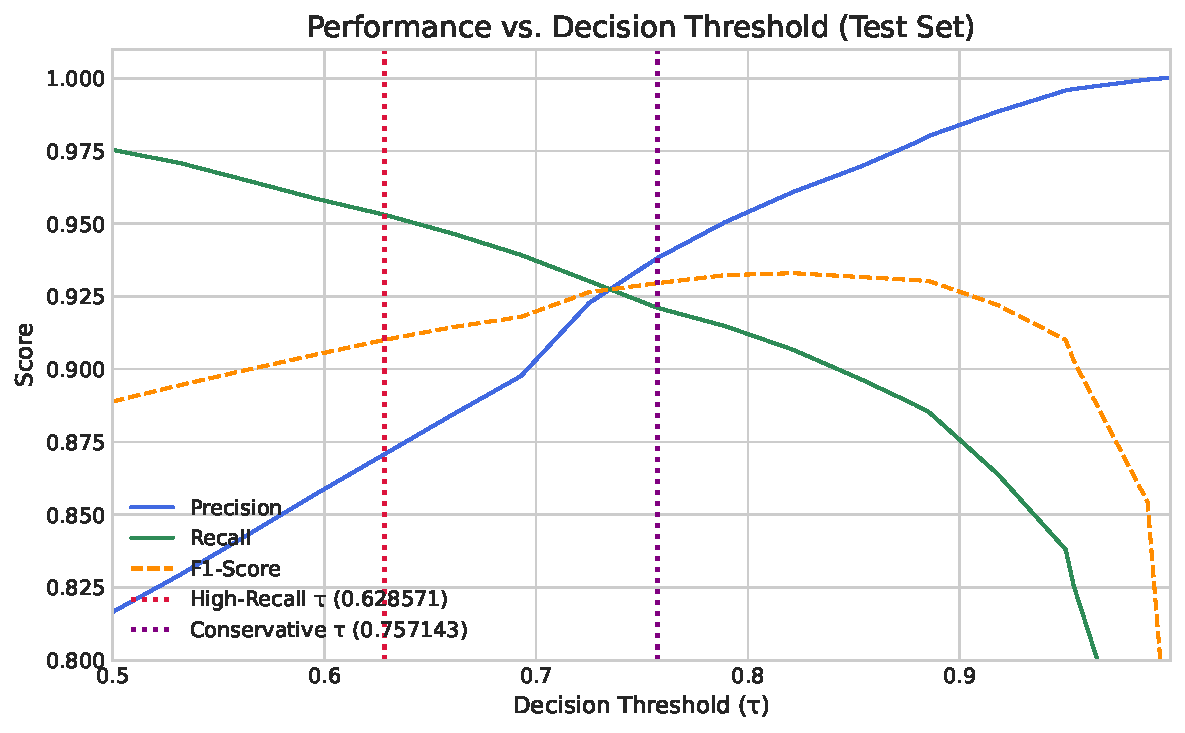
\includegraphics[width=\columnwidth]{fig_threshold_sweep.pdf}
  \caption{Precision, recall, and F1 versus threshold $\tau$ on the test set ($N{=}82{,}332$).
  Vertical markers indicate the two operating points: high–recall policy at $\tau{=}0.628571$
  and conservative point at $\tau{=}0.757143$. Thresholds evaluated on a discrete grid ($\Delta\tau{=}0.01$).}
  \label{fig:tau-sweep}
\end{figure}

\begin{figure}[t]
  \centering
  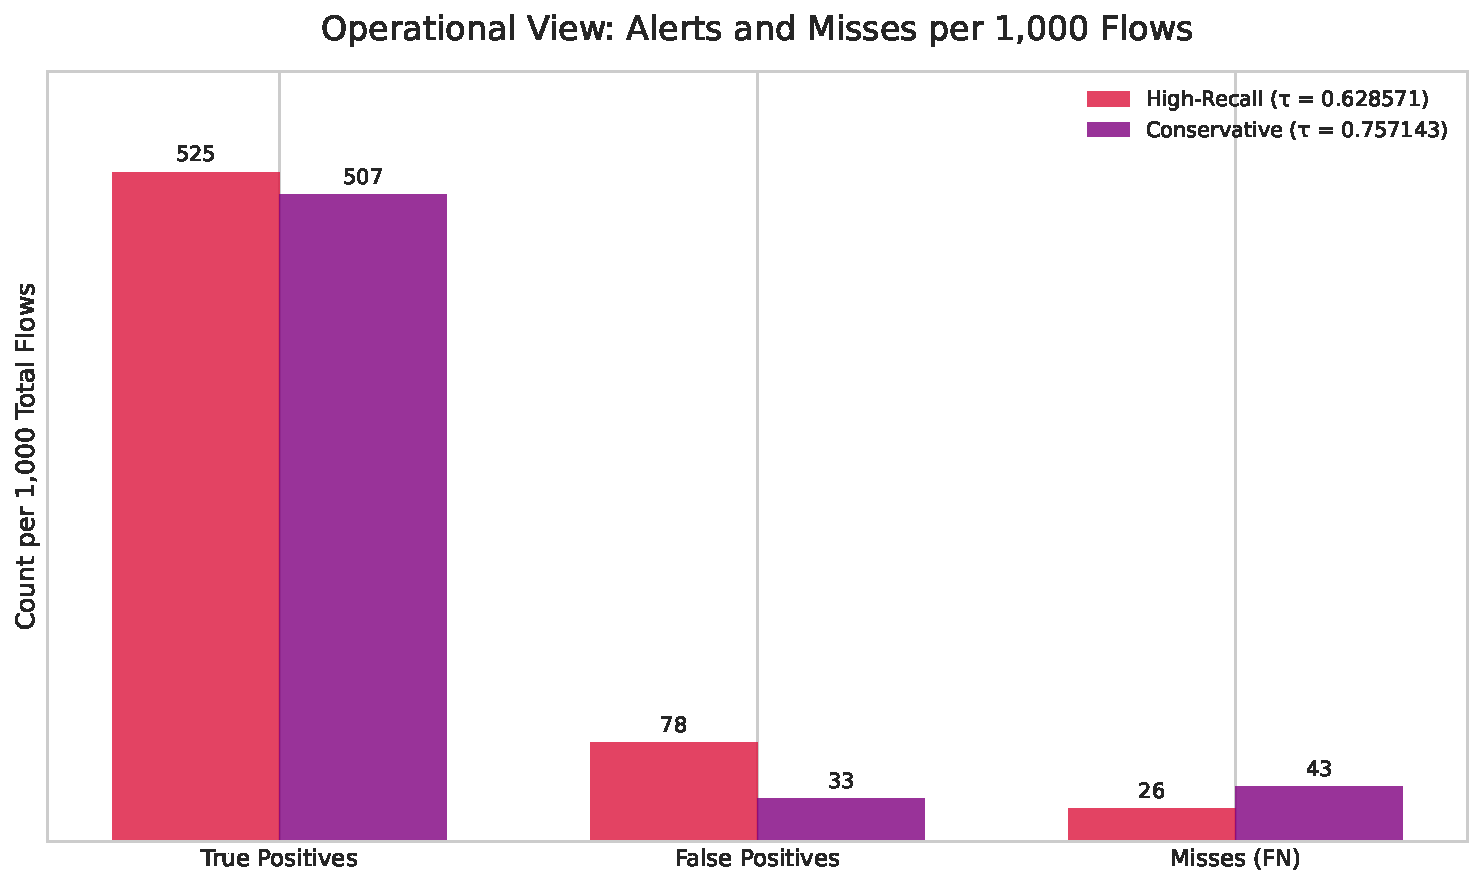
\includegraphics[width=\columnwidth]{fig_operational_per_1k.pdf}
  \caption{Operational view per 1{,}000 total flows at the two operating points on the test set
  ($N{=}82{,}332$; positives $45{,}332$, negatives $37{,}000$). High–recall ($\tau{=}0.628571$):
  $\text{TP}\approx525$, $\text{FP}\approx78$, $\text{FN}\approx26$; Conservative ($\tau{=}0.757143$):
  $\text{TP}\approx507$, $\text{FP}\approx33$, $\text{FN}\approx43$. Values rounded to nearest integer.}
  \label{fig:ops-1k}
\end{figure}

The high-recall regime minimizes missed detections ($\sim$47 per 1,000 positives) at the cost of more false alerts. The conservative regime reduces false alerts by $\sim$2.4$\times$ (175 $\to$ 74 per 1,000 negatives) but increases misses ($\sim$79 per 1,000 positives). Threshold governance of this form is increasingly recommended in IDS research to make cost trade-offs explicit and auditable \cite{zoghi2024}.

\subsection{Serving performance}
Following \texttt{05\_Deployment\_Optimization.ipynb}, we scored the full test batch (82,332 flows) in one call and measured wall-clock time and throughput, isolating model execution (no JSON/network).

\begin{table}[ht!]
\caption{Inference timing (full test batch: 82,332 flows).}
\label{tab:inference_timing}
\centering
\begin{tabular}{lrr}
\toprule
Artefact / Mode & Total time & Throughput (samples/s) \\
\midrule
XGBoost (CPU, inplace\_predict) & 43.4 ms & 1,896,013 \\
XGBoost (GPU, DMatrix) & 31.9 ms & 2,579,091 \\
XGBoost (GPU, CuPy + inplace\_predict) & 10.0 ms & 8,249,945 \\
ONNX Runtime (CPU) & 97.6 ms & 843,876 \\
\bottomrule
\end{tabular}
\end{table}

The GPU \texttt{inplace\_predict} path consistently achieved $\sim$8.25M flows/s. CPU ONNX was $\sim$2.25$\times$ slower than native CPU XGBoost, but still processed $\sim$0.84M flows/s—ample for real-time flow-level detection. Similar findings in prior UNSW-NB15 studies confirm XGBoost’s efficiency and robustness when tuned for both accuracy and runtime \cite{zoghi2022, pansari2024}.

\section{Discussion}
\subsection{Interpreting the results in a security context}
The tuned XGBoost classifier achieved strong detection performance on UNSW-NB15—ROC-AUC $\approx 0.98$ and F1 $\ge 0.90$ at operational thresholds. Similar work confirms that ensemble and boosting models are especially effective for balancing precision and recall on this dataset \cite{more2024, kocher2021}. The recall-constrained sweep shows that $\ge$95\% sensitivity can be enforced while keeping precision reasonable, which is critical for reducing the chance of missed intrusions in SOCs, where even a single false negative may be unacceptable \cite{krishna2024}. The conservative operating point provides a counterbalance, lowering analyst workload by cutting false alerts $\sim$2.4$\times$, but at the cost of more misses. Exposing the threshold via API metadata allows operators to retune without retraining. This is an operational governance control not often documented in IDS studies.

\subsection{Robustness and real-world resilience}
Beyond raw accuracy, the system includes resilience features: a deterministic preprocessing pipeline with schema contracts (preventing train–serve drift), recall-floor thresholding (auditable and adaptable under drift), and ONNX parity checks. Prior work stresses that robust IDSs require both statistical performance and deployment safeguards such as reproducibility and monitoring \cite{alani2021}. Still, UNSW-NB15 is a finite snapshot, and like others have noted, dataset artefacts and lack of evolving traffic may inflate results \cite{meftah2019}. Practical deployments must track drift (new services, adversary adaptation) and retrain periodically. Hybrid approaches (signatures + anomaly detection) are recommended to improve resilience \cite{sai2024}.

\subsection{Trade-offs: accuracy, latency, and operational complexity}
Threshold choice directly shapes risk and analyst capacity. At $\tau = 0.6286$, recall is maximised but false positives rise ($\sim$175 per 1,000 negatives). At $\tau = 0.7571$, false positives drop by $\sim$2.4$\times$ but misses increase. These trade-offs mirror broader findings: IDS deployment requires tuning models to balance analyst workload with acceptable risk \cite{merlin2024}.

Performance-wise, CPU XGBoost scored the test batch in 43.4 ms ($\sim$1.90M flows/s), while CPU ONNX was slower but remained real-time. GPU inference doubled throughput but adds operational complexity. Others confirm that scalable IDS must balance detection accuracy with low latency and infrastructure feasibility \cite{jose2024, prasad2022}. Kubernetes HPA offers burst handling, but larger clusters raise operational overhead. Operators must weigh high recall (coverage), GPU acceleration (throughput), and CPU ONNX (simplicity).

\subsection{Cloud deployment \& operations — discussion}
Our EKS deployment choices shape reliability, security, and cost in ways that extend beyond raw model quality.

\textbf{Boundary \& blast radius.} Exposing only the UI publicly while keeping the API cluster-internal narrows the attack surface and centralizes ingress control. The trade-off is that the UI becomes a chokepoint: if misconfigured, it could relay authenticated calls to the API. This argues for least-privilege secrets in the UI (scoped tokens, short TTL), rate-limiting/WAF at the UI endpoint, and audit trails tying each \texttt{/set\_threshold} or \texttt{/deploy\_registry} to an operator identity. Such layered defenses echo best practices for secure AWS/EKS workloads \cite{algarni2021}.

\textbf{Auth on health.} Early iterations guarded \texttt{/health} with the same Bearer policy as other routes to prevent probe backdoors, but this complicated liveness and readiness manifest design. The current implementation exempts \texttt{/health} from authentication, allowing standard Kubernetes HTTP probes to cleanly verify service availability without passing secrets. This aligns with microservice patterns where deep health checks are secure but top-level readiness endpoints are safely public.

\textbf{Autoscaling signal.} A CPU-based HPA aligns with the compute-bound ONNX Runtime path and scales appropriately under sustained load. But it lags on bursty traffic or serialization-heavy workloads, and ignores latency SLOs. If p95 latency becomes critical, request-rate, queue-depth, or custom latency metrics should drive scaling. Research on AI-driven autoscaling in EKS confirms that workload-aware signals improve reliability and cost efficiency compared to static CPU triggers \cite{thota2023}.

\textbf{Release discipline \& provenance.} Deploying SHA-tagged images and smoke-testing before rollout gives strong traceability and blocks most drift. Two lightweight hardenings: deploy by image digest (immutability end-to-end) and run a canary pod exercised by the Postman suite before full rollout. Because thresholds and bundles are externalized, rollbacks restore not just code but the exact model + $\tau$ pair. These practices align with resilient CI/CD frameworks in cloud-native deployments \cite{ashtagi2025}.

\textbf{Cost posture.} Scaling node groups to zero during idle periods reduces spend, but incurs cold-start latency (pulls, ORT warm-up). A pragmatic compromise is keeping one small UI replica up while scaling API pods from zero on demand. \texttt{LoadBalancer} services incur ELB costs; disabling the UI LB when not in use is another lever. Over the long term, private endpoints with identity-aware access may eliminate public exposure altogether. EKS architectural strategies emphasize cost-aware autoscaling and minimizing idle nodes to optimize spend \cite{mohammed2025}.

\textbf{Observability that matters.} High-yield signals include:
\begin{itemize}
    \item \textbf{Contract:} schema-mismatch rate and 422s at \texttt{/predict(\_proba)}, scaler/bundle load failures, bundle-hash drift.
    \item \textbf{Outcomes:} alerts per 1,000 flows, false-alerts per 1,000 negatives, score-distribution drift (label-free proxy).
    \item \textbf{Performance:} p50/p95 inference latency, throughput per replica, UI$\to$API error budgets.
    \item \textbf{Governance:} every threshold change and model reload logged with pre/post $\tau$, model digest, and operator identity.
\end{itemize}

\textbf{Provenance \& model governance.} MLflow logs parameters, metrics, and artefacts; the ONNX model can be promoted through the Model Registry and pulled by the service via registry-aware endpoints. This separation of experiment $\to$ registry $\to$ deployment makes changes auditable and rollbacks mechanical, echoing cloud-native MLOps patterns \cite{naayini2025}.

\subsection{Ethical and privacy considerations}
Flow telemetry reveals metadata about who communicated, when, and how much, this data that may qualify as personal under regimes such as GDPR/POPIA. Studies highlight that IDS research must consider privacy-preserving methods, lawful bases for processing, and safeguards against misuse \cite{rahman2024_synth}. Over-reliance on automation is risky: false positives can waste resources, while false negatives create false assurance. Transparent governance, however, documenting feature use, threshold policies, and auditable outcomes is essential for accountable IDS deployment. Ethical operation also requires human-in-the-loop oversight and clear boundaries to avoid mission creep or surveillance misuse.

\section{Conclusion}
We set out to close the gap between research-grade IDS models and operations-ready systems. Grounded on UNSW-NB15, we delivered a reproducible pipeline that yields a fixed 34-feature numeric schema with strict train–serve alignment; selected an operating point via a recall-constrained sweep; and demonstrated a champion XGBoost model that attains robust test performance at two auditable regimes (high-recall and conservative). The trained model is exported to ONNX with fixed I/O semantics and validated by smoke-level parity checks (same labels/metrics at the persisted $\tau$). We packaged the result as a token-authenticated FastAPI service with an operator Dash UI, versioned and promoted through MLflow (tracking + registry), and deployed to AWS EKS with SHA-pinned releases, CPU HPA, and CI-gated rollouts. The net effect is an IDS that is not only accurate but governable: measurable, reproducible, and adjustable without retraining.

\section{Future work}
To strengthen real-world resilience and operational safety, we see four high-leverage extensions:

\textbf{Drift detection \& calibration monitoring.} Track label-free shift via score-distribution divergence (PSI/JS) and add periodic ECE/Brier checks when labels are available. Trigger operator review or re-evaluation when drift exceeds thresholds. This aligns with concept-drift resilient IDS research, which shows that adaptive retraining is vital for effectiveness in dynamic networks \cite{andresini2021, alsuwat2023}.

\textbf{Retraining \& promotion loop.} Establish scheduled retraining on recent traffic with registry-gated promotion (Staging $\to$ Production), including automatic backtests at the current $\tau$. Provenance should tie each deployment to a specific model version + threshold pair. This echoes scalable MLOps practices for continuous model refresh and governance \cite{vijayan2024}.

\textbf{Canary deployments \& digest-pinned rollouts.} Roll out by image digest (immutability end-to-end) with a one-pod canary per service, tested by the smoke suite before widening. Add a lightweight probability-level parity check (max-|$ \Delta$|) between native and ONNX to detect subtle converter regressions. Canary release strategies are recommended in resilient CI/CD pipelines \cite{jana2022}.

\textbf{Domain naming \& access posture.} Introduce a private, identity-aware endpoint (or managed Ingress with mTLS/WAF) for the UI instead of a raw \texttt{LoadBalancer} hostname. Use separate tokens for UI$\to$API and CI/CD with short TTLs and rotation policies. Such hardened access models reflect modern deployment-shift mitigation approaches in IDS \cite{pawlicki2022}.

These steps build directly on the current system and would turn a robust, production-ready IDS into an operationally resilient platform that adapts gracefully under drift and load while remaining auditable end-to-end.

\bibliographystyle{unsrtnat} % numeric, ordered by first citation
\bibliography{refs}          % your .bib file

\end{document}

